\section{U-Net}
\label{sec:Chapter22}

\begin{figure}[H]
\centering
\definecolor{boxcol}{rgb}{0.7,0.8,1.0}
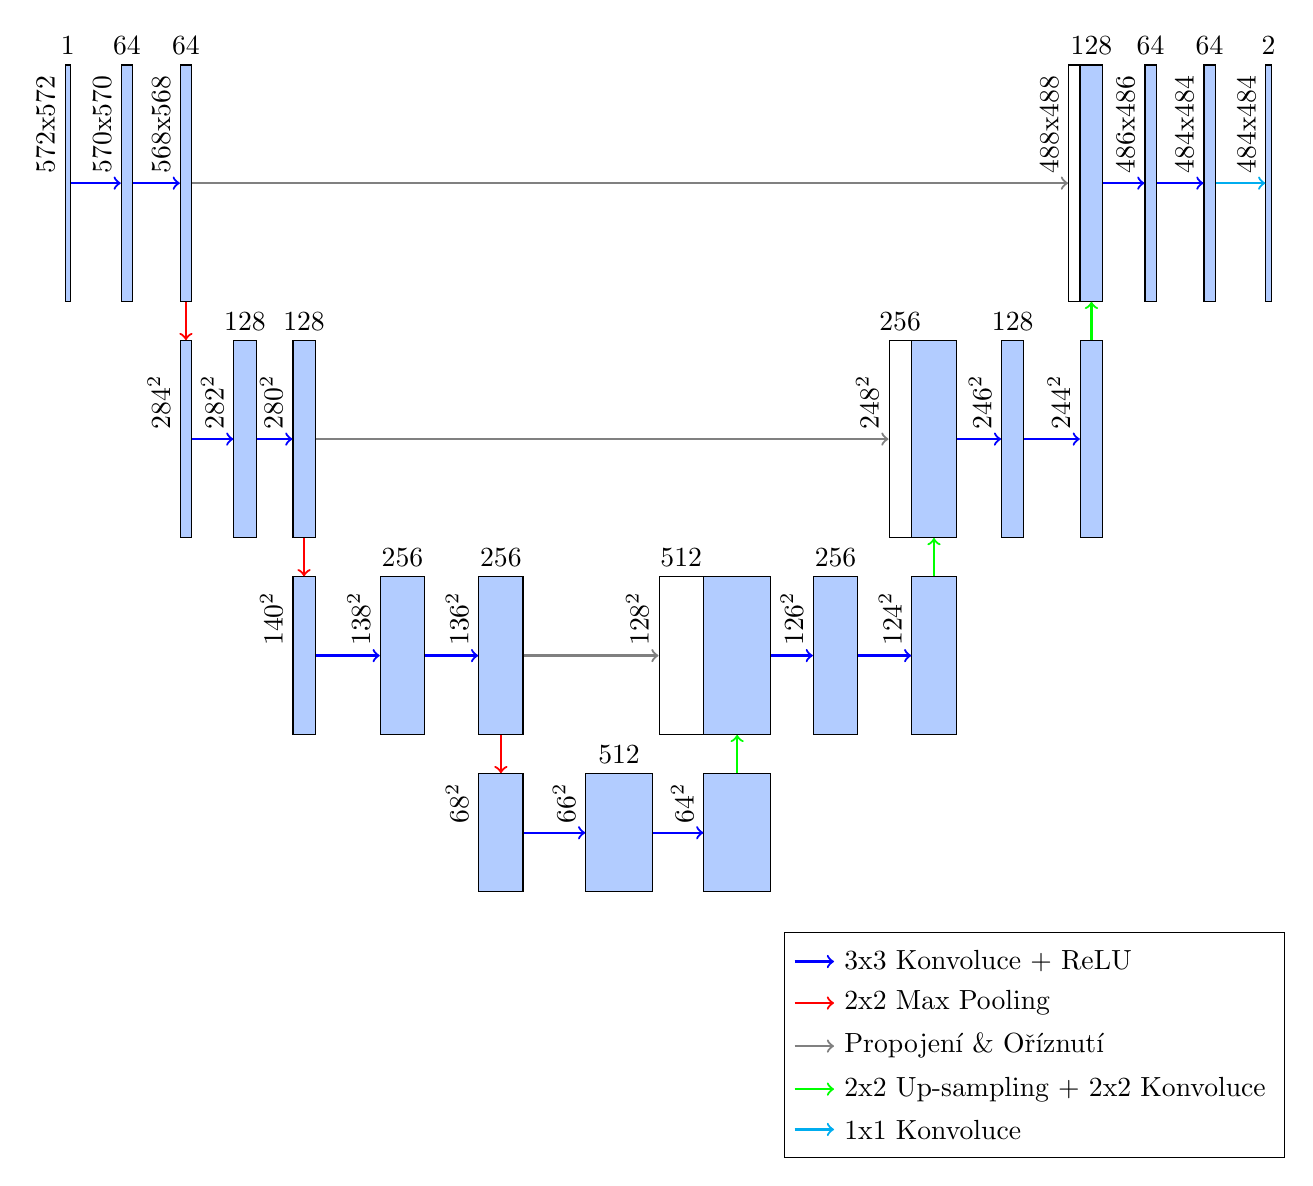
\begin{tikzpicture}[
    box/.style={draw, inner sep=2pt, fill=boxcol, minimum height=30mm},
    skipbox/.style={draw, inner sep=2pt, fill=white, minimum height=30mm},
    rotate label/.style={anchor=south west, rotate=90, xshift=+0mm},
    redarrow/.style={->, draw=red, thick},
    grayarrow/.style={->, draw=gray, thick},
    bluearrow/.style={->, draw=blue, thick},
    greenarrow/.style={->, draw=green, thick},
    cyanarrow/.style={->, draw=cyan, thick}
  ]
  
  \coordinate (e00p) at (0,20); 
  \coordinate (e01p) at (0.75, 20);
  \coordinate (e02p) at (1.5, 20);
  
  \coordinate (e10p) at (1.5, 16.75);
  \coordinate (e11p) at (2.25, 16.75);
  \coordinate (e12p) at (3.0, 16.75);

  \coordinate (e20p) at (3, 14);
  \coordinate (e21p) at (4.25, 14);
  \coordinate (e22p) at (5.5, 14);

  \coordinate (b0p) at (5.5, 11.75);
  \coordinate (b1p) at (7.0, 11.75);
  \coordinate (b2p) at (8.5, 11.75);

  \coordinate (s0p)  at (7.79, 14);
  \coordinate (d00p) at (8.5,  14); 
  \coordinate (d01p) at (9.75, 14);
  \coordinate (d02p) at (11.0, 14);

  \coordinate (s1p)  at (10.57, 16.75);
  \coordinate (d10p) at (11.0, 16.75);
  \coordinate (d11p) at (12.0, 16.75);
  \coordinate (d12p) at (13.0, 16.75);

  \coordinate (s2p) at (12.78, 20);
  \coordinate (d20p) at (13.0, 20);
  \coordinate (d21p) at (13.75, 20);
  \coordinate (d22p) at (14.5, 20);
  \coordinate (d23p) at (15.25, 20);

  % Encoder
  \node[box, label=above:1, label={[rotate label]left:572x572}, inner sep=1pt] (e00) at (e00p) {};
  \node[box, label=above:64, label={[rotate label]left:570x570}] (e01) at (e01p) {};
  \node[box, label=above:64, label={[rotate label]left:568x568}] (e02) at (e02p) {};

  \node[box, label={[rotate label]left:$284^2$}, inner sep=2pt, minimum height=25mm] (e10) at (e10p) {};
  \node[box, label=above:128, label={[rotate label]left:$282^2$}, inner sep=4pt, minimum height=25mm] (e11) at (e11p) {};
  \node[box, label=above:128, label={[rotate label]left:$280^2$}, inner sep=4pt, minimum height=25mm] (e12) at (e12p) {};

  \node[box, label={[rotate label]left:$140^2$}, inner sep=4pt, minimum height=20mm] (e20) at (e20p) {};
  \node[box, label=above:256, label={[rotate label]left:$138^2$}, inner sep=8pt, minimum height=20mm] (e21) at (e21p) {};
  \node[box, label=above:256, label={[rotate label]left:$136^2$}, inner sep=8pt, minimum height=20mm] (e22) at (e22p) {};

  % Bottleneck
  \node[box, label={[rotate label]left:$68^2$}, inner sep=8pt, minimum height=15mm] (b0) at (b0p) {};
  \node[box, label=above:512, label={[rotate label]left:$66^2$}, inner sep=12pt, minimum height=15mm] (b1) at (b1p) {};
  \node[box, label={[rotate label]left:$64^2$}, inner sep=12pt, minimum height=15mm] (b2) at (b2p) {};

  % Decoder
  \node[skipbox, label=above:512, label={[rotate label]left:$128^2$}, inner sep=8pt, minimum height=20mm] (s0) at (s0p) {};
  \node[box, inner sep=12pt, minimum height=20mm] (d00) at (d00p) {};
  \node[box, label=above:256, label={[rotate label]left:$126^2$}, inner sep=8pt, minimum height=20mm] (d01) at (d01p) {};
  \node[box, label={[rotate label]left:$124^2$}, inner sep=8pt, minimum height=20mm] (d02) at (d02p) {};

  \node[skipbox, label=above:256, label={[rotate label]left:$248^2$}, inner sep=4pt, minimum height=25mm] (s1) at (s1p) {};
  \node[box, inner sep=8pt, minimum height=25mm] (d10) at (d10p) {};
  \node[box, label=above:128, label={[rotate label]left:$246^2$}, inner sep=4pt, minimum height=25mm] (d11) at (d11p) {};
  \node[box, label={[rotate label]left:$244^2$}, inner sep=4pt, minimum height=25mm] (d12) at (d12p) {};


  \node[skipbox, label={[rotate label]left:488x488}, inner sep=2pt, minimum height=30mm] (s2) at (s2p) {};
  \node[box, label=above:128, inner sep=4pt, minimum height=30mm] (d20) at (d20p) {};
  \node[box, label=above:64, label={[rotate label]left:486x486}, inner sep=2pt, minimum height=30mm] (d21) at (d21p) {};
  \node[box, label=above:64, label={[rotate label]left:484x484}, inner sep=2pt, minimum height=30mm] (d22) at (d22p) {};
  \node[box, label=above:2, label={[rotate label]left:484x484}, inner sep=1pt, minimum height=30mm] (d23) at (d23p) {};


  % Connect the boxes to form "U" shape
  \draw[bluearrow] (e00) -- (e01);
  \draw[bluearrow] (e01) -- (e02);
  \draw[redarrow] (e02) -- (e10);
  
  \draw[bluearrow] (e10) -- (e11);
  \draw[bluearrow] (e11) -- (e12);
  \draw[redarrow] (e12) -- (e20);
  
  \draw[bluearrow] (e20) -- (e21);
  \draw[bluearrow] (e21) -- (e22);
  \draw[redarrow] (e22) -- (b0);
  
  \draw[bluearrow] (b0) -- (b1);
  \draw[bluearrow] (b1) -- (b2);
  \draw[greenarrow] (b2) -- (d00);

  \draw[bluearrow] (d00) -- (d01);
  \draw[bluearrow] (d01) -- (d02);
  \draw[greenarrow] (d02) -- (d10);
  
  \draw[bluearrow] (d10) -- (d11);
  \draw[bluearrow] (d11) -- (d12);
  \draw[greenarrow] (d12) -- (d20);
  
  \draw[bluearrow] (d20) -- (d21);
  \draw[bluearrow] (d21) -- (d22);
  \draw[cyanarrow] (d22) -- (d23);

  \draw[grayarrow] (e02) -- (s2);
  \draw[grayarrow] (e12) -- (s1);
  \draw[grayarrow] (e22) -- (s0);


  \matrix [draw,below left, yshift=-0.5cm] at (current bounding box.south east) {
      \draw [bluearrow] (0,0) -- (0.5,0) node[right] {3x3 Konvoluce + ReLU}; \\
      \draw [redarrow] (0,0) -- (0.5,0) node[right] {2x2 Max Pooling}; \\
      \draw [grayarrow] (0,0) -- (0.5,0) node[right] {Propojení \& Oříznutí}; \\
      \draw [greenarrow] (0,0) -- (0.5,0) node[right] {2x2 Up-sampling + 2x2 Konvoluce}; \\
      \draw [cyanarrow] (0,0) -- (0.5, 0) node[right] {1x1 Konvoluce}; \\
  };
  
\end{tikzpicture}

\caption[Příkladná architektura sítě U-Net]{Architektura sítě U-Net s 3 bloky enkodéru a dekodéru. Vytvořeno podle \cite{unet}. }
\label{fig:unetdiagram}

\end{figure}

\textbf{U-Net} je architektura CNN poprvé představena v roce 2015 v literatuře \cite{unet}. Jedná se o architekturu konvoluční neuronové sítě, hojně využívanou pro segmentační úlohy, avšak je používána i pro lokalizační, klasifikační a další problémy analýzy obrazu \cite{unet_success}. Architektura sítě U-Net spočívá ve třech sémantických částí, kde každá část zaznamenává jiné typy informací získaných z vstupních obrazů - enkodér, krk (ang. bottleneck) a dekodér. Závěrečná, čtvrtá vrstva je specificky navržena a uzpůsobena pro konkrétní úkol, pro který je síť navržena.

\subsection{Stavba CNN sítě}
\label{subsec:Chapter221}

\textbf{Enkodér} sestává ze sémantických vrstev konvolučních bloků, kde každou sémantickou vrstvou sítě se zdvojnásobuje počet filtrů a rozměr obrazu se naopak dělí dvěma pomocí 2x2 max pooling vrstev na koncích bloků enkodéru. Cílem enkodéru je zachytit kontextuální rysy vstupního obrazu \cite{unet_success}.

\textbf{Krk (ang. bottleneck)} je prvek uprostřed sítě U-Net, která propojuje enkodér na jeho konci a dekodér na jeho počátku. Tato část sítě obsahuje nejmenší velikost obrazu, zato maximální počet filtrů v konvolučních vrstvách.

\textbf{Dekodér} je symetrická složka k enkodéru, kde každou sémantickou vrstvou sítě se počet filtrů naopak dělí dvěma. Vstupy do sémantických vrstev dekodérů z předchozích částí sítě předchází 2x2 vrstvy, kterým se v orig. literatuře říká up-convolution. Ve skutečnosti se jedná o vrstvu 2x2 typu up-sampling, následovanou 2x2 konvoluční vrstvou. Dekodér zachycuje vysoko-úrovňovější rysy a také je zodpovědný za finální lokalizaci \cite{unet_success}.

Všechny tyto 3 extrační části zpravidla obsahují dvě 3x3 konvoluční vrstvy, zpravidla s odsazením typu valid padding a (1, 1) krokem (ang. stride), aplikovány následně po sobě s ReLU aktivační funkcí, obdobně jako v původní architektuře \cite{unet}. Postupem síť U-Net zlepšuje své receptivní pole, a v hlubších vrstvách se zlepšuje v zachycování sémantických a kontextuálních informací. Ovšem postupem síť také ztrácí lokalizační informace, pro které byly do sítě U-Net přidány také skokové propojení (tj. skip connection) mezi odpovídajícími vrstvami enkodéru a dekodéru \cite{unet_success}.

Těmito fundamentálními částmi sítě U-Net vzniká vizuální podoba písmenu 'U', odkud pochází jeho název. Velikost sítě U-Net díky své symetrické a sémanticky jednoznačné architektuře může být zmenšena či zvětšena. Například v obrázku \ref{fig:unetdiagram} je síť sestavena ze 3 bloku enkodéru a dekodéru, avšak často se používá i velikost se 4 bloky (jako např. v originální literatuře \cite{unet}) nebo jiným počtem.

\subsection{Výstup CNN sítě}
\label{subsec:Chapter222}

Na konci sítě U-Net se nachází výstupní vrstva s několika filtry. Počet těchto filtrů odpovídá počtu tříd, které chceme v obrázku segmentovat. V případě binární segmentace (obdobně jako na obrázku \ref{fig:unetdiagram}), kde rozlišujeme mezi popředím a pozadím, se používají 2 filtry. Každý z těchto filtrů produkuje mapu pravděpodobností pro jednotlivé třídy.

Následně se aplikuje softmax funkce na výstupy těchto filtrů. Softmax je použit proto, aby se výstupy převedly na spojitou pravděpodobnostní distribuci, která umožňuje jednoznačně určit, zda pixel patří do popředí nebo pozadí. Softmax zajistí, že součet pravděpodobností pro každý pixel a pro všechny třídy bude roven 1, což umožňuje interpretovat výstupy jako pravděpodobnostní příslušnosti k jednotlivým třídám.

Je důležité poznamenat, že v případě více než dvou tříd segmentace se počet filtrů na konci U-Net odpovídajícím způsobem zvýší, aby každá třída měla svůj vlastní filtr. Následně se pro trénink sítí pro podobné segmentační úlohy, ať už binární nebo několika třídové, používají například ztrátové funkce z řad cross-entropy \cite{unet}.

\subsection{Využití}
\label{subsec:Chapter223}

U-Net se stal hojně používanou architekturou, kterou dnes můžeme nalézt i např. v biomedicínském inženýrství \cite{unet_success} nebo i difuzních modelech pro syntézi vysoko-rozměrových obrázků \cite{stablediffusion}.

Za rok 2022 se sítě U-Net oproti předchozím letům velmi rozšířily, a např. v medicíně byly využity převážně pro segmentaci a klasifikaci. Avšak sítě U-Net byly schopny být aplikovány i na podobné problémy počítačového vidění zahrnující, ale neomezující se na rekonstrukce, detekce, deformační obrazová registrace\footnote{Problém mapovaní/transformace lehce deformovaného či posunutého obrazu na obraz druhý \cite{unet_registration}.}, odšumění či další. V roce 2022 dosáhl U-Net dle zmíněné literatury téměř 3 tisíc vědeckých článků za rok, což je například trojnásobně vyšší než před dvěma lety v roce 2020 \cite{unet_success}.

\endinput